%!TEX program = lualatex
%
% Main document
% ===========================================================================
% This is part of the document "Project documentation template".
% Authors: brd3, kaa1
%

%---------------------------------------------------------------------------
\documentclass[
	a4paper,					% paper format
	10pt,							% fontsize
	twoside,					% double-sided
	openright,				% begin new chapter on right side
	notitlepage,			% use no standard title page
	parskip=half,			% set paragraph skip to half of a line
]{scrreprt}					% KOMA-script report
%---------------------------------------------------------------------------

\raggedbottom
\KOMAoptions{cleardoublepage=plain}			% Add header and footer on blank pages
\providecommand{\versiondate}{2019-06-13}

% Load Standard Packages:
%---------------------------------------------------------------------------
\usepackage[standard-baselineskips]{cmbright}

\usepackage[ngerman,english]{babel}										% english hyphenation
%\usepackage[latin1]{inputenc}  							% Unix/Linux - load extended character set (ISO 8859-1)
%\usepackage[ansinew]{inputenc}  							% Windows - load extended character set (ISO 8859-1)
\usepackage[T1]{fontenc}											% hyphenation of words with ä, ö and ü
\usepackage{textcomp}													% additional symbols
\usepackage{ae}																% better resolution of Type1-Fonts 
\usepackage{fancyhdr}													% simple manipulation of header and footer 
\usepackage{etoolbox}													% color manipulation of header and footer
\usepackage{graphicx}                      		% integration of images
\usepackage{float}														% floating objects
\usepackage{caption}													% for captions of figures and tables
\usepackage{booktabs}													% package for nicer tables
\usepackage{tocvsec2}													% provides means of controlling the sectional numbering
\usepackage{dirtree}


\usepackage{nameref}
\usepackage{listings}
\usepackage{listings, color}

\definecolor{dkgreen}{rgb}{0,0.6,0}
\definecolor{gray}{rgb}{0.5,0.5,0.5}
\definecolor{mauve}{rgb}{0.58,0,0.82}

\lstset{
  language=scala,
  basicstyle=\footnotesize,
  keywordstyle=\color{blue},
  commentstyle=\color{dkgreen},
  numbers=left,
  %frame=single, % Border around box
  numbersep=-7pt,
  numberstyle=\color{gray},
  stringstyle=\color{mauve}
}

\usepackage{soul}
\definecolor{lightgray}{rgb}{0.90, 0.90, 0.90}
\newcommand{\code}[1][\sethlcolor{lightgray}\hl]{#1}
\newcommand\mypound{\scalebox{0.8}{\raisebox{0.4ex}{\#}}}
%---------------------------------------------------------------------------

% Load Math Packages
%---------------------------------------------------------------------------
\usepackage{amsmath}                    	   	% various features to facilitate writing math formulas
\usepackage{amsthm}                       	 	% enhanced version of latex's newtheorem
\usepackage{amsfonts}                      		% set of miscellaneous TeX fonts that augment the standard CM
\usepackage{amssymb}													% mathematical special characters
\usepackage{exscale}													% mathematical size corresponds to textsize
%---------------------------------------------------------------------------

% Package to facilitate placement of boxes at absolute positions
%---------------------------------------------------------------------------
\usepackage[absolute]{textpos}
\setlength{\TPHorizModule}{1mm}
\setlength{\TPVertModule}{1mm}
%---------------------------------------------------------------------------					

% Definition of Colors
%---------------------------------------------------------------------------
\RequirePackage{color}                          % Color (not xcolor!)
\definecolor{linkblue}{rgb}{0,0,0.8}            % Standard
\definecolor{darkblue}{rgb}{0,0.08,0.45}        % Dark blue
\definecolor{bfhgrey}{rgb}{0.41,0.49,0.57}      % BFH grey
%\definecolor{linkcolor}{rgb}{0,0,0.8}     			% Blue for the web- and cd-version!
\definecolor{linkcolor}{rgb}{0,0,0}        			% Black for the print-version!
%---------------------------------------------------------------------------

% Hyperref Package (Create links in a pdf)
%---------------------------------------------------------------------------
\usepackage[
	pdftex,ngerman,bookmarks,plainpages=false,pdfpagelabels,
	backref = {false},										% No index backreference
	colorlinks = {true},                  % Color links in a PDF
	hypertexnames = {true},               % no failures "same page(i)"
	bookmarksopen = {true},               % opens the bar on the left side
	bookmarksopenlevel = {0},             % depth of opened bookmarks
	bookmarksopenlevel = {0},             % depth of opened bookmarks
	pdftitle = {Formal Verification in Scala},	   	% PDF-property
	pdfauthor = {brd3},        					  % PDF-property
	pdfsubject = {LaTeX Template},        % PDF-property
	linkcolor = {linkcolor},              % Color of Links
	citecolor = {linkcolor},              % Color of Cite-Links
	urlcolor = {linkcolor},               % Color of URLs
]{hyperref}
%---------------------------------------------------------------------------

% Set up page dimension
%---------------------------------------------------------------------------
\usepackage{geometry}
\geometry{
	a4paper,
	left=28mm,
	right=15mm,
	top=30mm,
	headheight=20mm,
	headsep=10mm,
	textheight=242mm,
	footskip=15mm
}
%---------------------------------------------------------------------------

% Makeindex Package
%---------------------------------------------------------------------------
\usepackage{makeidx}                         		% To produce index
\makeindex                                    	% Index-Initialisation
%---------------------------------------------------------------------------

% Glossary Package
%---------------------------------------------------------------------------
% the glossaries package uses makeindex
% if you use TeXnicCenter do the following steps:
%  - Goto "Ausgabeprofile definieren" (ctrl + F7)
%  - Select the profile "LaTeX => PDF"
%  - Add in register "Nachbearbeitung" a new "Postprozessoren" point named Glossar
%  - Select makeindex.exe in the field "Anwendung" ( ..\MiKTeX x.x\miktex\bin\makeindex.exe )
%  - Add this [ -s "%tm.ist" -t "%tm.glg" -o "%tm.gls" "%tm.glo" ] in the field "Argumente"
%
% for futher informations go to http://ewus.de/tipp-1029.html
%---------------------------------------------------------------------------
% \usepackage[nonumberlist]{glossaries}
% \makeglossaries
% \include{database/glossary}
%---------------------------------------------------------------------------

% Intro:
%---------------------------------------------------------------------------

% KAI
\newcommand{\todo}[1]{{\par \large \color{red}#1}}


\begin{document}                              	% Start Document
\settocdepth{subsection}														% Set depth of toc
\pagenumbering{roman}														
%---------------------------------------------------------------------------

\providecommand{\heading}{Experiments in Formal Verification of Scala Code}		%  Insert Title of Thesis here					% Titel der Arbeit aus Datei titel.tex lesen
% \input{leader/version}				% Versionsnummer und -datum aus Datei version.tex lesen

% Set up header and footer
%---------------------------------------------------------------------------
\makeatletter
\patchcmd{\@fancyhead}{\rlap}{\color{bfhgrey}\rlap}{}{}		% new color of header
\patchcmd{\@fancyfoot}{\rlap}{\color{bfhgrey}\rlap}{}{}		% new color of footer
\makeatother

\fancyhf{}																		% clean all fields
\fancypagestyle{plain}{												% new definition of plain style	
	\fancyfoot[OR,EL]{\footnotesize \thepage} 	% footer right part --> page number
	\fancyfoot[OL,ER]{\footnotesize \heading}	% footer even page left part 
}

\renewcommand{\chaptermark}[1]{\markboth{\thechapter.  #1}{}}
\renewcommand{\headrulewidth}{0pt}				% no header stripline
\renewcommand{\footrulewidth}{0pt} 				% no bottom stripline

\pagestyle{plain}
%---------------------------------------------------------------------------


% Title Page and Abstract
%---------------------------------------------------------------------------
%
% Project documentation template
% ===========================================================================
% This is part of the document "Project documentation template".
% Authors: brd3, kaa1
%

\begin{titlepage}


% BFH-Logo absolute placed at (28,12) on A4 and picture (16:9 or 15cm x 8.5cm)
% Actually not a realy satisfactory solution but working.
%---------------------------------------------------------------------------
\setlength{\unitlength}{1mm}
\begin{textblock}{20}[0,0](28,12)
	
\includegraphics[scale=1.0]{images/BFH_Logo_B.png}
\end{textblock}

% Institution / titel / subtitel / authors / experts:
%---------------------------------------------------------------------------
\begin{flushleft}

\vspace*{21mm}

\fontsize{26pt}{40pt}\selectfont 
\heading				\\							% Read heading from file leader/title.tex
\vspace{2mm}

\fontsize{16pt}{24pt}\selectfont\vspace{0.3em}
% Place your subheading here 			\\				% Insert subheading
\vspace{5mm}

\fontsize{10pt}{12pt}\selectfont
\textbf{Bachelor Thesis} \\		% Insert text
\vspace{7mm}

% Abstract (eingeben):
%---------------------------------------------------------------------------
\begin{textblock}{150}(28,100)
% \fontsize{10pt}{12pt}\selectfont
% [Insert short text (abstract) if desired] \\ 
% This document serves as a template for the compilation of reports according to the guidelines of the BFH. The template is written in LATEX and supports the automatic writing of various directories, references, indexing and glossaries. This small text is a summary of this document with a length of 4 to max. 8 lines. \\ 
% The cover picture may be turned on or off in the lines 157/158 of the file template.tex.
\end{textblock}

\begin{textblock}{150}(28,225)
\fontsize{10pt}{17pt}\selectfont
\begin{tabbing}
xxxxxxxxxxxxxxx\=xxxxxxxxxxxxxxxxxxxxxxxxxxxxxxxxxxxxxxxxxxxxxxx \kill
Degree course:	\> Computer Science	\\		% insert name of degree course
Authors:		\> Anna Doukmak, Ramon Boss		\\					% insert names
Tutor:	\> Prof. Dr. Kai Brünnler		\\							% insert names
%Constituent:	\> [Wwwww AG]					\\							% insert names
%Expert:		\> [Dr.~Zzzz Zzzz]				\\							% insert names
Date:			\> \versiondate					\\							% read from file leader/version.tex
\end{tabbing}

\end{textblock}
\end{flushleft}

\begin{textblock}{150}(28,280)
\noindent 
\color{bfhgrey}\fontsize{9pt}{10pt}\selectfont
Berner Fachhochschule | Haute \'ecole sp\'ecialis\'ee bernoise | Bern University of Applied Sciences
\color{black}\selectfont
\end{textblock}


\end{titlepage}

%
% ===========================================================================
% EOF
%
		% activate for frontpage without picture
% \include{leader/frontpage_with_picture}		% activate for frontpage with picture
% \include{leader/versions}
\cleardoubleemptypage
\setcounter{page}{1}
\cleardoublepage
\phantomsection 
\addcontentsline{toc}{chapter}{Abstract}
\chapter*{Abstract}
\label{chap:abstract}

In this thesis we try to verify some properties of Bitcoin-S.

First, we look at some theory about formal verification, Stainless -- a verification tool and Bitcoin-S -- an open source implementation of the Bitcoin protocol.

Then, we try to verify that a non-coinbase transaction should not generate new coins.
We create a transaction and check it in Bitcoin-S.
After some time we realize that it is not possible with the current tools and the given time.
But because we familiarized us with the Bitcoin-S code we find a bug and send a bug fix to the Bitcoin-S project.

So we verify a less interesting property of Bitcoin-S.
There is a datatype Satoshis that represents bitcoins. We verify that the addition of Satoshis with zero results in the same amount of Satoshis.
Even this needs many changes in the code that we go through step-by-step.

Finally, we see that software should be written with verification tools in mind, because otherwise the code possibly must be rewritten when it comes to verification.

\cleardoubleemptypage
%---------------------------------------------------------------------------

% Table of contents
%---------------------------------------------------------------------------
\tableofcontents
\cleardoublepage
%---------------------------------------------------------------------------

% Main part:
%---------------------------------------------------------------------------
\pagenumbering{arabic}

\chapter{Introduction}
\label{chap:introduction}

The longer and more complex a source code is, the more difficult it is to verify its correctness.
There are different approaches to show the correctness of a program.
One of them is formal verification.
In contrast to testing, where only predefined inputs are tested, with formal verification all possible inputs are covered.
The correctness of a program is analyzed relative to its formal specification.
Formal specification is a mathematical description of a software behavior that can be used by the verification tool to verify the code.
We will see an example of a formal specification shortly.

In this work we use the verification framework Stainless to verify parts of the code of Bitcoin-S, a Scala implementation of the Bitcoin protocol.
In the following we look at the main aspects of formal verification with Stainless and properties of Bitcoin-S we want to verify.


\section{Formal Verification with Stainless}
\label{sec:stainless}

Stainless is developed by "Lab for Automated Reasoning and Analysis" (LARA) at EPFL's School of Computer and Communication Sciences.
Using this framework we can verify the correctness of Scala programs.
The following overview of the framework is taken from the section \href{https://epfl-lara.github.io/stainless/intro.html}{Introduction} of the Stainless documentation \cite{Stainless:documentation}.

Stainless statically verifies that a program satisfies a given specification and that a program will not crash at runtime.
The framework covers all possible inputs and finds a counter examples for possible failures in a program which violate the given specification.

The main functions used to write a specification are \textit{require} and \textit{ensuring}.

With \textit{require} we define a precondition of a function, which we want to verify.
\textit{require} is placed at the beginning of the function body.
\textit{require} specifies, if the parameter of the function holds against a certain condition.

With \textit{ensuring}, we define the postcondition of a function.
\textit{ensuring} is placed at the end of the function after the body.
\textit{ensuring} specifies, if the return value or the result of the function satisfies a certain condition.

On invoking Stainless, it tries to prove that the postcondition always holds, assuming the given precondition does hold.

The following example demonstrates a simple formal specification for the function calculating a factorial.
This is a modified example from the section \href{https://epfl-lara.github.io/stainless/intro.html}{Introduction} of the Stainless documentation \cite{Stainless:documentation}, so Stainless reports an error verifying it.
\begin{lstlisting}[language=Scala]
  def factorial(n: Int): Int = {
      require(n >= 0)
      if (n == 0) {
        1
      } else {
        n * factorial(n - 1)
      }
  } ensuring(res => res >= 0)
\end{lstlisting}

It recursively calculates the factorial of an integer number.
The input of the function is constrained with \textit{require} to a non-negative value.
The result should also be non-negative.
Thus, Stainless will verify whether the result of the factorial calculation is non-negative for all non-negative inputs.

Stainless can produce 3 outcomes of postcondition verification: \textit{valid}, \textit{invalid} and \textit{unknown}.
If the postcondition is \textit{valid} Stainless could prove that for any inputs constrained in the precondition, the postcondition always holds.
Reporting the postcondition as \textit{invalid} the framework could find at least one counterexample which satisfies the precondition but violates the postcondition.
If Stainless is unable to prove the postcondition or find a counterexample it reports the outcome \textit{unknown}.
In this case a timeout or an internal error occurred.
Furthermore, Stainless checks for calls in the code to the function with invalid arguments violating the precondition.
For example if we invoke factorial with a negative number it reports \textit{invalid}.

Let's return to our incorrect example with factorial.
Stainless reports the following result for the factorial verification from our example:
\begin{figure}[H]
	\centering
		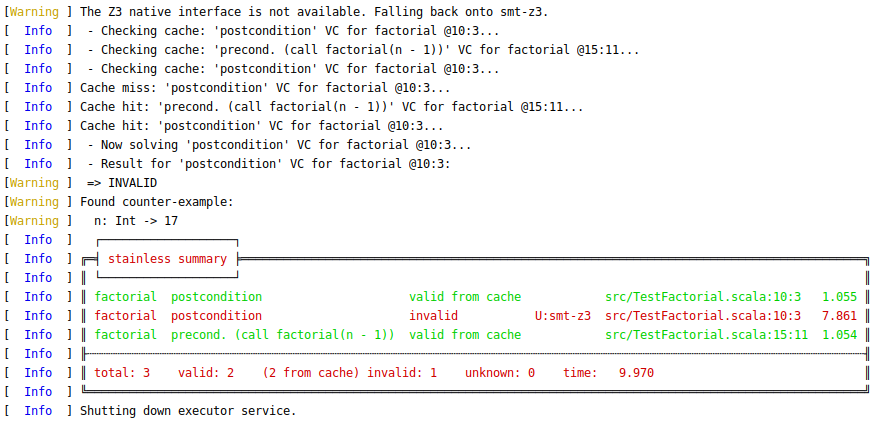
\includegraphics[scale=0.5]{images/output1.png}
	\caption{Output of Stainless verification for calculating factorial of Int number}
	\label{fig:output1}
\end{figure}

Stainless disproves the postcondition and gives the number 17 as a counterexample.
Due to an overflow in the 32 bit Int the result becomes a negative value.
The program would work correct by changing the type from Int to BigInt.

Stainless supports only a subset of Scala. \todo{Anna It supports blabla, in particular it supports not blablabla. (check class with var)}

\todo{why does stainless use its own BigInt etc?}

They call this Pure Scala.
You can find the specification of Pure Scala on the Stainless documentation website \cite{Stainless:documentation} in the section \href{https://epfl-lara.github.io/stainless/purescala.html}{Pure Scala}.

In addition, Stainless has its own library with annotations, reimplementation of some core data types, collections and input-output functions and more.
Some of them are described on the website in the section \href{https://epfl-lara.github.io/stainless/library.html}{Stainless Library}.
There are more details about the library in the source code of Stainless on GitHub \cite{Stainless:github} in the folder \href{https://github.com/epfl-lara/stainless/tree/master/frontends/library/stainless}{\textit{frontends/library/stainless}}.

Stainless verifies Scala programs using SMT (satisfiability modulo theories) solvers. 


\section{The Properties to Verify}

Bitcoin-S is a large project found on GitHub implementing many functionalities.
In this work we look at two of them, namely the \nameref{property_1} and the \nameref{property_2} described shortly.
Thus, we go through the relevant code parts to verify those properties, look at some challenges with Stainless and see why we should write software with verification in mind.
In order to be able to verify Bitcoin-S, we have to rewrite parts of it in the subset of Scala supported by Stainless.


\subsection{No-Inflation Property}
\label{property_1}

The decision to verify this property was inspired by the bug found in Bitcoin Core in September 2018  \cite{cve201817144} which allowed to spend the same unspent transaction output (UTXO) in a transaction multiple times.
Hence, new coins could be created out of the air.
Thus, we try to verify the property, that a non-coinbase transaction cannot generate new coins.
Let's name it the \nameref{property_1}.

As we can see later in chapter \ref{chap:verify_check}, we must rewrite a huge part of the code implementing this property.
This reimplementation into Pure Scala needs a lot of time.
So, we adjust the plan and verify another functionality of Bitcoin-S.
Nevertheless, during the analysis of the \nameref{property_1} we look at a bug in Bitcoin-S found during this work and see the code changes for the bugfix in section \ref{sec:bugfix}. 


\subsection{Addition-with-Zero Property}
\label{property_2}

In Bitcoin-S there is a class \texttt{Satoshis} representing an amount of bitcoins.
We look at the verification of the addition of Satoshis with zero Satoshis.
This operation should result in the same amount of Satoshis.
Let's call it the \nameref{property_2}.

Using Stainless, we see the successful verification of this property.
But the process of the verification with the tool requires many changes in the code, so that Stainless can accept it.
We look at all needed modifications in chapter \ref{chap:verify_add}.

\chapter{Trying to Verify the No-Inflation Property}
\label{chap:verify_check}

This chapter describes the part of Bitcoin-S needed to verify the \nameref{property_1} described before.
We are going to create a transaction and show the relevant parts of the method \texttt{checkTransaction}, where transactions are checked against some properties.
Then, we will see the bug in Bitcoin-S found during this work and its fix.
In the end we see why the \nameref{property_1} needed to be changed to the \nameref{property_2}.


\section{Creation of a Transaction}

Some code in this section is copied or adapted from the Bitcoin-S-Core transaction builder example \cite{BitcoinSCore:txbuilderexample}.
Bitcoin-S-Core has a bitcoin transaction builder class with the following constructor:
\begin{lstlisting}[language=scala]
  BitcoinTxBuilder(
    destinations: Seq[TransactionOutput], // where to send the money
    utxos: BitcoinTxBuilder.UTXOMap,      // unspent transaction outputs
    feeRate: FeeUnit,                     // fee rate per byte
    changeSPK: ScriptPubKey,              // where to send the change
    network: BitcoinNetwork               // bitcoin network information
  ): Future[BitcoinTxBuilder]
\end{lstlisting}

The return type Future does not make sense here, since the implementation calls either Future.successful or Future.fromTry which returns an already resolved Future.
This might be for future purposes.

Now we create a transaction.

First, we need some money.
Thus, we create a fake transaction with one single output.
This transaction can be parsed from the bitcoin network, but we create one manually in order to see this process.
\begin{lstlisting}[language=scala]
  val privKey = ECPrivateKey.freshPrivateKey
  val creditingSPK = P2PKHScriptPubKey(pubKey = privKey.publicKey)

  val amount = Satoshis(Int64(10000))

  val utxo = TransactionOutput(currencyUnit = amount, scriptPubKey = creditingSPK)

  val prevTx = BaseTransaction(
    version = Int32.one,
    inputs = List.empty,
    outputs = List(utxo),
    lockTime = UInt32.zero
  )
\end{lstlisting}

On line one and two we create a new keypair to sign the next transaction and have a scriptPubKey where the bitcoins are.
This is our keypair.
So the money is transferred to our public key.
Line four specifies the amount of satoshis we have in the transaction.
Then we create the actual transaction from line 6 to 13.

Now that we have some bitcoins, we create the new transaction where we want to spend them.

First, we need some out points.
They point to outputs of previous transactions.
We use the index zero, because the previous transaction has only one output that becomes the first index zero.
If there were two previous outputs, the second output would become the index 1 and so on.
\begin{lstlisting}[language=scala]
  val outPoint = TransactionOutPoint(prevTx.txId, UInt32.zero)

  val utxoSpendingInfo = BitcoinUTXOSpendingInfo(
    outPoint = outPoint,
    output = utxo,
    signers = List(privKey),
    redeemScriptOpt = None,
    scriptWitnessOpt = None,
    hashType = HashType.sigHashAll
  )

  val utxos = List(utxoSpendingInfo)
\end{lstlisting}

This utxos are the inputs of our transaction.

Second, we need destinations to spend the bitcoins to.
For the sake of convenience we create only one.
\begin{lstlisting}[language=scala]
  val destinationAmount = Satoshis(Int64(5000))

  val destinationSPK = P2PKHScriptPubKey(pubKey = ECPrivateKey.freshPrivateKey.publicKey)

  val destinations = List(
    TransactionOutput(currencyUnit = destinationAmount, scriptPubKey = destinationSPK)
  )
\end{lstlisting}

We spend 5000 satoshis to the newly created random public key.

Finally, we define the fee rate in satoshis per one byte transaction size as well as some bitcoin network parameters.
The bitcoin network parameters are not important, so we use some static values normally used when testing.
\begin{lstlisting}[language=scala]
  val feeRate = SatoshisPerByte(Satoshis.one)

  val networkParams = RegTest // some static values for testing
\end{lstlisting}

Now lets build the transaction with those data.
\begin{lstlisting}[language=scala]
  val txBuilderF: Future[BitcoinTxBuilder] = BitcoinTxBuilder(
    destinations = destinations, // where to send the money
    utxos = utxos,               // unspent transaction outputs
    feeRate = feeRate,           // fee rate per byte
    changeSPK = creditingSPK,    // where to send the change
    network = networkParams      // bitcoin network information
  )

  val signedTxF: Future[Transaction] = txBuilderF
    .flatMap(_.sign)                       // call sign on the transaction builder
    .map {
      (tx: Transaction) => println(tx.hex) // transaction in hex for the bitcoin network
    }
\end{lstlisting}

\todo{ramon: change code to get an actual transaction, completely understand and explain the code}

Line one to seven creates a transaction builder which is then signed on line ten.
We can now use our transaction object on line twelve.
For example, after calling \emph{hex} on it, we can send the returned string to the bitcoin network.


\section{Validation of a Transaction}

Bitcoin-S offers a function called \emph{checkTransaction} located in the ScriptInterpreter object.
This is its type signature:
\begin{lstlisting}[language=scala]
  checkTransaction(transaction: Transaction): Boolean
\end{lstlisting}

\todo{kai: code zeigen}

We can pass a transaction and it returns a Boolean indicating whether the transaction is valid or not.
So for example when we pass the transaction we built before the returned value would be true, because it's a valid transaction.
It might not be accepted by the bitcoin network but for a transaction on its own it's valid.
We can not check context with it, because we can only pass one transaction.

There are several checks in checkTransaction.
For example, it checks if there is either no input or no output.
In this case we get false.

The relevant part for the bug we found:
\begin{lstlisting}[language=scala]
  val prevOutputTxIds = transaction.inputs.map(_.previousOutput.txId)
  val noDuplicateInputs = prevOutputTxIds.distinct.size == prevOutputTxIds.size
\end{lstlisting}

It gathers all transaction ids referenced by the out points.
When we call \emph{distinct} on the returned list, we get a list with duplicate removed.
If the size of the new list is the same as the size of the old, we know that there was no duplicate transaction id, because, as said, distinct removes the duplicates.


\section{Fixing a Bug in Bitcoin-S}
\label{sec:bugfix}

We can see that there is a bug in the checkTransaction function from before, recognized and fixed through this work.

\begin{figure}[H]
	\centering
		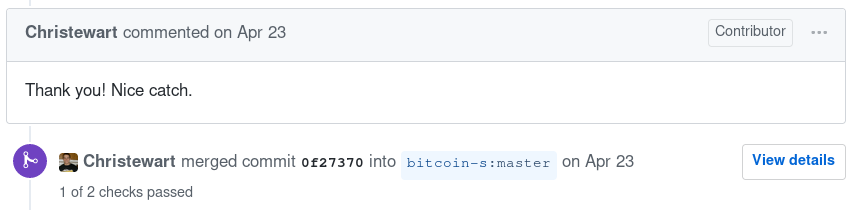
\includegraphics[scale=0.5]{images/bitcoin-s-pr-comment.png}
	\caption{Nice catch comment on our PR \#435 on GitHub}
	\label{fig:output1}
\end{figure}

Here is the relevant code of checkTransaction again:
\begin{lstlisting}[language=scala]
  val prevOutputTxIds = transaction.inputs.map(_.previousOutput.txId)
  val noDuplicateInputs = prevOutputTxIds.distinct.size == prevOutputTxIds.size
\end{lstlisting}

What happens if we have two TransactionOutPoints (previousOutputs) with a different index but referencing the same Transaction ID (txId)?

According to the Bitcoin protocol this is possible.
A transaction can have multiple outputs that should be referenceable by the next transaction.
So this is clearly a bug.

What should not be possible is a transaction referencing the same output twice.
This bug occurred in Bitcoin Core known as CVE-2018–17144 which was patched on September 18, 2018. \cite{cve201817144}

Here, Bitcoin-S did a bit too much and marked all transaction as invalid, if they referenced the same transaction twice.
The fix is, to check on TransactionOutPoint instead of TransactionOutPoint.txId, because TransactionOutPoint contains the txId as well as the output index it references.
So in pseudo code, we check on the tuple (tx, index) instead of (tx).
The fixed code:
\begin{lstlisting}[language=scala]
  val prevOutputs = transaction.inputs.map(_.previousOutput)
  val noDuplicateInputs = prevOutputs.distinct.size == prevOutputs.size
\end{lstlisting}

Since TransactionOutPoint is a case class and Scala has a built in == for case classes there is no need to implement TransactionOutPoint.==.
\begin{figure}[H]
	\centering
		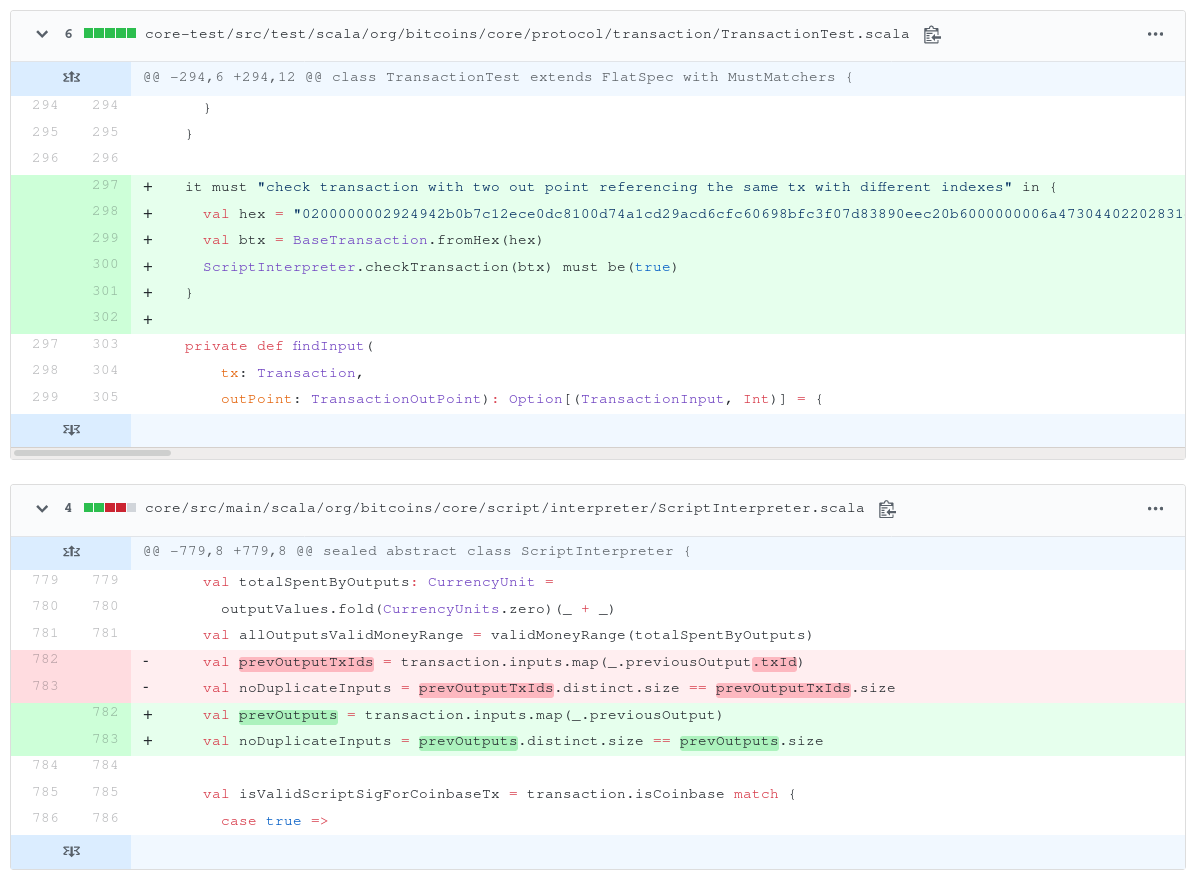
\includegraphics[scale=0.396]{images/bitcoin-s-pr.png}
	\caption{Line changes for PR \#435 from GitHub}
	\label{fig:output1}
\end{figure}

This was fixed in \href{https://github.com/bitcoin-s/bitcoin-s/pull/435}{pull request \mypound435} on GitHub at April 23, 2019, through this work along with a unit test to prevent this bug from appearing again in the future.


\section{Adjusting No-Inflation Property}

\todo{anna: what does it mean to integrate}

Trying to integrate Stainless in Bitcoin-S caused a lot of troubles, mainly because of version conflicts.
For more details see chapter \ref{chap:appendix_arb}.

After integrating Stainless in Bitcoin-S, there were many errors.
It takes too much time to fix them all so it should be easier to extract the classes needed for the \texttt{checkTransaction} function.
\todo{anna: which errors?}

The extracted code has more than 1500 lines.
After running Stainless on it, it still throws a huge bunch of errors about what Stainless can not reason about.
After fixing some of those errors, there appear new ones.
So this would require changing nearly everything of the extracted code.

Let's adjust the property from the \nameref{property_1} to the \nameref{property_2}, because there is not enough time to fix all these errors and write the verification.
This is way less interesting to verify but gives still many insights in what needs to be done to verify some parts of Bitcoin-S and other source code.

So let's look at the \nameref{property_2}.

\chapter{Towards Verifying the Addition-with-Zero Property}
\label{chap:verify_add}



After realizing that it would consume too much time to rewrite the Bitcoin-S code and even the extracted part with checkTransaction, the smallest unit in Bitcoin-S-Core that is worthwhile to verify was extracted.
This could be the addition of two CurrencyUnits.
To make it even easier, the addition of CurrencyUnits with zero.
CurrencyUnits is an abstract class in Bitcoin-S, representing currencies like Satoshis.

\section{Extracting the relevant Code}

\todo{ramon: write this section}
\todo{ramon: keep close to original code}
\todo{ramon: for every transformation: before and after}
\todo{ramon,anna: for every transformation: why does it preserve the semantics}
\todo{ramon,anna: add comments}
\todo{ramon,anna: explain what the code does and why}

Here we can see the extracted code needed for the addition of CurrencyUnits:
\lstinputlisting[language=scala]{../code/currsniporig/src/main/scala/code/initial/Code.scala}

The additions' signature looks like this:
\begin{lstlisting}[language=scala]
  +(c: CurrencyUnit): CurrencyUnit
\end{lstlisting}

When we run Stainless on this code (without any properties to prove), it throws the following errors:
{\footnotesize\begin{verbatim}
  [ Error  ] Code.scala:41:1: Objects cannot extend classes or implement traits,
             use a case object instead
           object Int64 extends BaseNumbers[Int64] {
           ^^^^^^^^^^^^^^^^^^^^^^^^^^^^^^^^^^^^^^^^^...
  [ Error  ] Code.scala:60:3: Stainless doesn't support abstract type members
              type A
              ^^^^^^
  [ Error  ] Code.scala:77:33: Only literal arguments are allowed for BigInt.
              def toBigInt: BigInt = BigInt(toLong)
                                            ^^^^^^
  [ Error  ] Code.scala:84:1: Objects cannot extend classes or implement traits,
             use a case object instead
            object Satoshis extends BaseNumbers[Satoshis] {
            ^^^^^^^^^^^^^^^^^^^^^^^^^^^^^^^^^^^^^^^^^^^^^^^...
  [  Info  ] Shutting down executor service.
\end{verbatim}}

So let's see how we can fix those errors.


\section{Turning Object into Case Object}

Stainless output:
{\footnotesize\begin{verbatim}
  [ Error  ] Code.scala:41:1: Objects cannot extend classes or implement traits,
             use a case object instead
           object Int64 extends BaseNumbers[Int64] {
           ^^^^^^^^^^^^^^^^^^^^^^^^^^^^^^^^^^^^^^^^^...
  [ Error  ] Code.scala:84:1: Objects cannot extend classes or implement traits,
            use a case object instead
            object Satoshis extends BaseNumbers[Satoshis] {
            ^^^^^^^^^^^^^^^^^^^^^^^^^^^^^^^^^^^^^^^^^^^^^^^...
\end{verbatim}}

Here, we can just change the objects from object to case object.
Stainless recommendation is to use objects for modules and case objects as algebraic data types.

This is due to the internal design of Scala.
It's possible to reason about case object but not about object.
This needs a fundamental knowledge of Scala and some functional paradigms that should not be part of this thesis.
The \href{https://github.com/epfl-lara/stainless/issues/520}{issue \mypound520} on Stainless GitHub gives some thoughts, if you want to know more.


\section{Getting Rid of Abstract Type Member}

Stainless output:
{\footnotesize\begin{verbatim}
  [ Error  ] Code.scala:60:3: Stainless doesn't support abstract type members
              type A
              ^^^^^^
\end{verbatim}}

This should be easy to rewrite by using generics instead of an abstract type, right?
Unfortunately not.
The problem is, CurrencyUnit uses one of its implementing classes: Satoshis.

Simplified code.
\begin{lstlisting}[language=scala]
  sealed abstract class CurrencyUnit {
    type A

    def +(c: CurrencyUnit): CurrencyUnit =
      Satoshis(satoshis.underlying + c.satoshis.underlying)

    protected def underlying: A
  }

  sealed abstract class Satoshis extends CurrencyUnit {
    override type A = Int64
  }
\end{lstlisting}

What happens, if we typify CurrencyUnit with A, meaning to make it generic with type A?

Satoshis extends CurrencyUnit with type Int64, so it would be of type CurrencyUnit[Int64].
That's too specific, because the return type of the addition is then CurrencyUnit[Int64] not CurrencyUnit[A].
Maybe the Bitcoin-S developers should reimplement this part and not use Satoshis directly.

Since there is no easy way to fix it and the code should stay as much as possible the original, we just remove the abstract type and set it to Int64.
This limits the verification a bit, but as we only want to verify the addition in satoshis, that's OK.


\section{Replacing the BigInt Constructor Argument With A String Literal}

Stainless output:
{\footnotesize\begin{verbatim}
  [ Error  ] Code.scala:77:33: Only literal arguments are allowed for BigInt.
              def toBigInt: BigInt = BigInt(toLong)
                                            ^^^^^^
\end{verbatim}}

As described before, Stainless supports only a subset of Scala.
The BigInt from the Stainless library is a bit restricted.
One such restriction is, that BigInt does not support dynamic BigInt construction.
Thus, the constructor parameter of BitInt must be a literal argument.

Again, a simplified code version.
\begin{lstlisting}[language=scala]
  sealed abstract class Satoshis extends CurrencyUnit { 
    def toBigInt: BigInt = BigInt(toLong)
    def toLong: Long = underlying.toLong
  }
\end{lstlisting}

This would be really hard to refactor, because Bitcoin-S tries to be as dynamic as possible so it can be used with cryptocurrencies other than bitcoins.
Maybe it could be impossible, because they need to parse dynamic values from the bitcoin network.

Luckily, we can use toBigInt on the field \texttt{underlying} directly instead of toLong.
So, instead of converting the underlying to Long and back to BigInt we convert underlying directly to BigInt.

After fixing all Stainless errors, a new error appears.


\section{Getting Rid of Special Generics}

Stainless output:
{\footnotesize\begin{verbatim}
  [ Error  ] Code.scala:7:30: Unknown type parameter type T
             sealed abstract class Number[T <: Number[T]]
                                         ^^^^^^^^^^^^^^
\end{verbatim}}

This is a missing feature in Stainless.
It does not support upper type boundaries on the class itself.
To track this, \href{https://github.com/epfl-lara/stainless/issues/519}{issue \mypound519} was created on GitHub during this work.
\begin{lstlisting}[language=scala]
  sealed abstract class Number[T <: Number[T]] extends BasicArithmetic[T]  
\end{lstlisting}

Despite this, in order to be able to continue, we make this a concrete type by replacing T with Int64.
Int64,  because Satoshis uses only Int64.
There are other number types like UInt16 but for our property we don't need them.

Now, there are two new errors.


\section{Getting Rid of Concrete Type}

Stainless output:
{\footnotesize\begin{verbatim}
  [Warning ] Code.scala:9:3: Could not extract tree in class: type A =
             BigInt (class scala.reflect.internal.Trees$TypeDef)
             type A = BigInt
             ^^^^^^^^^^^^^^^
\end{verbatim}}

This is easy.
We just replace all occurrence of A with BigInt, since A is not overwritten in an implementing class.
This is not the exact same code, because an implementing class can not override A anymore but that's fine for our verification.

This was a missing feature in Stainless that was fixed on Mai 28, 2019 with \href{https://github.com/epfl-lara/stainless/pull/470}{pull request \mypound470} on GitHub.
Now it should work without this change.


\section{Replacing the BigInt \&-Function With Bound Check}
\label{sec:bound_check}

Stainless output:
{\footnotesize\begin{verbatim}
  [ Error  ] Code.scala:22:14: Unknown call to & on result (BigInt) with arguments
             List(Number.this.andMask) of type List(BigInt)
            require((result & andMask) == result,
                    ^^^^^^^^^^^^^^^^
\end{verbatim}}

Due to the restrictions on BigInt, we can not use the \& function either.
Simplified code:
\begin{lstlisting}[language=scala]
  sealed abstract class Number extends BasicArithmetic[Int64] {
    def andMask: BigInt

    override def +(num: Int64): Int64 = apply(checkResult(underlying + num.underlying))

    private def checkResult(result: BigInt): BigInt = {
      require((result & andMask) == result, "Result was out of bounds, got: " + result)
      result
    }
  }
\end{lstlisting}

This is a bounds check.
It checks if the result of the addition is in range of the specified type, which is now the hard coded Int64.

So, we can replace the \& mask with a bound check whether the result is in range of Long.MinValue and Long.MaxValue, because Int64 has the same 64-bit range as Long.
Again the code gets a bit more static and it's not the exact same code anymore.

Running Stainless produces again new errors.


\section{Extracting Private Inner Classes}

Stainless output:
{\footnotesize\begin{verbatim}
  [Warning ] Code.scala:90:3: Could not extract tree in class: case private
             class SatoshisImpl extends Satoshis with Product with Serializable {
\end{verbatim}}

Stainless can not extract the private class inside the object.
Bitcoin-S uses this a lot, because they separate the class from its implementation.
Simplified:
\begin{lstlisting}[language=scala]
  object Int64 extends BaseNumbers[Int64] {
    private case class Int64Impl(underlying: BigInt) extends Int64 
  }
\end{lstlisting}

This is easy to fix.
We just extract the private class out of the object.
This is not exactly the same code, because other classes in the same file could now access the private class.
But for our property it does not change anything.

Now we get some weird warnings about require.


\section{Removing Second Parameter of Require}

Stainless output:
{\footnotesize\begin{verbatim}
  [Warning ] Code.scala:51:3: Could not extract tree in class: scala.this.Predef
             .require(Int64Impl.this.underlying.>=(math.this.BigInt.long2bigInt(
             -9223372036854775808L)), "Number was too small for a int64, got: "
             .+(Int64Impl.this.underlying)) (class scala.reflect.internal.Trees$Apply)
            require(underlying >= -9223372036854775808L,
            ^^^^^^^^^^^^^^^^^^^^^^^^^^^^^^^^^^^^^^^^^^^^...
  [Warning ] Code.scala:53:3: Could not extract tree in class: scala.this.Predef
             .require(Int64Impl.this.underlying.<=(math.this.BigInt.long2bigInt(
             9223372036854775807L)), "Number was too big for a int64, got: "
             .+(Int64Impl.this.underlying)) (class scala.reflect.internal.Trees$Apply)
            require(underlying <= 9223372036854775807L,
            ^^^^^^^^^^^^^^^^^^^^^^^^^^^^^^^^^^^^^^^^^^^...
  [ Error  ] checkResult$0 depends on missing dependencies: require$1.
\end{verbatim}}

Seems like Stainless does not support the second string parameter of require or at least it throws a warning about it.
We can safely remove the string parameters from the requires, since they only serve as error messages.

A new error appears.


\section{Rewriting BigInt Comparison with Long}

Stainless output:
{\footnotesize\begin{verbatim}
  [ Error  ] inv$4 depends on missing dependencies: long2bigInt$0.
\end{verbatim}}

This error is hard to understand, but we can see that there is a missing Long to BigInt conversion.
So we search for all Long values in the code.
\begin{lstlisting}[language=scala]
  private case class Int64Impl(underlying: BigInt) extends Int64 {
    require(underlying >= -9223372036854775808L)
    require(underlying <= 9223372036854775807L)
  }
\end{lstlisting}

Looks like it can not compare a BigInt with a Long value.
We can easily convert this Long value to a BigInt with a string literal parameter by passing these numbers as strings to the BigInt constructor.

Finally, we get some output from Stainless about the verification in the code.
{\footnotesize\begin{verbatim}
[...]
[Warning ]  => INVALID
[Warning ] Found counter-example:
[Warning ]   thiss: { x: Object | @unchecked isNumber(x) } -> Int64Impl(0)
[Warning ]   num: { x: Object | @unchecked isInt64(x) }    -> Int64Impl(9223372036854775808)
[...]
[  Info  ] +  precond. (call checkResult(thiss, underlying(thiss) + u ...)  invalid  Code.scala:16:45
[...]
[  Info  ] total: 5  valid: 4  (4 from cache) invalid: 1  unknown: 0  time:  1.317
\end{verbatim}}

This shows that there is an invalid specification in checkResult and Stainless prints a counterexample for it.

Let's ignore this for a moment and write the specification for the \nameref{property_2}.


\section{Writing Specification for the Property}

As specified, our verification must only support addition with zero.
So we restrict the parameter to be zero in the precondition.
\begin{lstlisting}[language=scala]
  require(c.satoshis == Satoshis.zero)
\end{lstlisting}

We ensure the result is the same value as \emph{this} in the postcondition.
\begin{lstlisting}[language=scala]
  ensuring(res => res.satoshis == this.satoshis)
\end{lstlisting}

We can use equals (==) directly on Satoshis, because it is a case class.
The addition will now look like this:
\begin{lstlisting}[language=scala]
  override def +(c: CurrencyUnit): CurrencyUnit = {
    require(c.satoshis == Satoshis.zero)
    Satoshis(satoshis.underlying + c.satoshis.underlying)
  } ensuring(res => res.satoshis == this.satoshis)
\end{lstlisting}

That's all we need to verify our addition.

Now we will look into the previous error.


\section{Propagating Require}

There is another problem with Bitcoin-S.
Bitcoin-S-Core uses require as a fail-fast method whereas Stainless needs it to verify the code.

The Stainless output again:
{\footnotesize\begin{verbatim}
  [Warning ] Found counter-example:
  [Warning ]   thiss: { x: Object | @unchecked isNumber(x) } -> Int64Impl(0)
  [Warning ]   num: { x: Object | @unchecked isInt64(x) }    -> Int64Impl(9223372036854775808)
\end{verbatim}}

Corresponding code:
\begin{lstlisting}[language=scala]
  sealed abstract class Number extends BasicArithmetic[Int64] {
    override def +(num: Int64): Int64 = apply(checkResult(underlying + num.underlying))

    private def checkResult(result: BigInt): BigInt = {
      require(
        result <= BigInt("9223372036854775807")
        && result >= BigInt("-9223372036854775808")
      )
      result
    }
  }
\end{lstlisting}

But how does Stainless find a counter example ignoring the require in checkResult?
Since Stainless is a static verification tool, it tests every possibility.
So it can use a number bigger than the maximum Int64 and pass it to the addition.
The require in checkResult fails.

Thus, we need to add the restriction from checkResult to the addition too.
\begin{lstlisting}[language=scala]
  override def +(num: Int64): Int64 = {
    require(
          num.underlying <= BigInt("9223372036854775807")
      &&  num.underlying >= BigInt("-9223372036854775808")
      && this.underlying <= BigInt("9223372036854775807")
      && this.underlying >= BigInt("-9223372036854775808")
    )
    apply(checkResult(underlying + num.underlying))
  }
\end{lstlisting}

Stainless finds another counter example:
{\footnotesize\begin{verbatim}
  [Warning ] Found counter-example:
  [Warning ]   num: { x: Object | @unchecked isInt64(x) }    -> Int64Impl(1)
  [Warning ]   thiss: { x: Object | @unchecked isNumber(x) } ->
                 Int64Impl(9223372036854775807)
\end{verbatim}}

Sure, when adding one to the maximum Int64 the require does not hold anymore.
Since we do only allow zero as a parameter, the easiest way is to restrict it to zero here too.


\section{Result}

Finally, everything is green and correctly verified.
\begin{figure}[H]
	\centering
		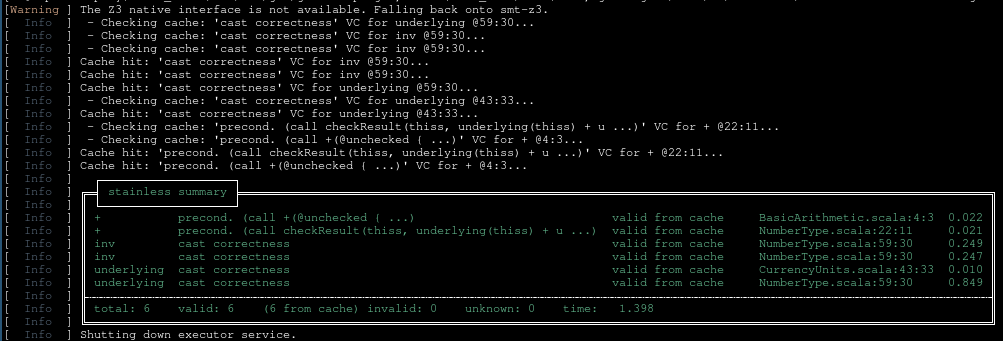
\includegraphics[scale=0.45]{images/final_verify_output.png}
	\caption{Output of Stainless verification for addition with 0 of Bitcoin-S-Cores CurrencyUnit}
	\label{fig:output1}
\end{figure}

The verified code.
\lstinputlisting[language=scala]{../code/currsniporig/src/main/scala/code/end/Code.scala}

But is it really the original code that we verified?
And why did we have to change that much?
This and other questions will be answered in the next chapter.

\chapter{Practical Challenges with Stainless}
\label{chap:appendix_arb}

In this chapter we look at the practical challenges that could occur by using Stainless.
Since Stainless is still in development and there is no 1.x release there might still be breaking changes and improvements fixing problems described now.


\section{sbt vs JAR}

We can either use the sbt plugin or a JAR file to check code with Stainless.

Invoking the JAR on our source code Stainless will verify it.
If we have a bigger project, this becomes really tricky, because we must pass all files needed including the dependencies.
This is in contrast to the sbt plugin, where we can integrate Stainless in our compilation process.
When we call compile, Stainless verifies the code and stops the compilation if the verification fails.

Having a static version configured in the sbt build file, every developer has the same Stainless features available.
This should prevent incompatibility with new or deprecated features when we use different plugins.

So the sbt plugin has clear advantages over the JAR file since its integrated directly.
We do not have to download it manually and find the right version and if we bump the version we can just edit it in the build file and every developer is on the same version again.

However, currently there are some drawbacks.
For example the sbt plugin does not always report errors.
We will see more about that shortly.


\section{Integration into Bitcoin-S}

During this work, Stainless updated the sbt plugin to support sbt 1.2.8 from 0.13.17 and Scala 2.12.8 from 2.11.12.
So this section might be out of date now.

Stainless requires and Scala recommends Java SE Development Kit 8.
Newer Java versions won't work.

To use the latest version of the sbt tool you have to build it locally.
You can run \code{sbt universal:stage} in the cloned Stainless git repository.
This generates \emph{frontends/scalac/target/universal/stage/bin/stainless-scalac}.

Bitcoin-S-Core uses sbt 1.2.8 and Scala 2.12.8, while Stainless sbt plugin is on sbt 0.13.17 and Scala 2.11.12.

Sbt introduced new features in the 1.x release used by Bitcoin-S.
Most of them can be written the sbt 0.13.17 way.

The bigger problem is, due to the different Scala and sbt versions, the following error after trying to go in a sbt shell:
\begin{verbatim}
  [warn] There may be incompatibilities among your library dependencies; run 'evicted'
         to see detailed eviction warnings.
  [error] java.lang.NoClassDefFoundError: sbt/SourcePosition
  ...
  Project loading failed: (r)etry, (q)uit, (l)ast, or (i)gnore?
\end{verbatim}

Downgrading Bitcoin-S sbt version to 0.13.17 fixes the error but then it can not load some libraries only compiled for newer versions.
So this would take too much time to fix and changes the Bitcoin-S code inadvertently.

The next approach is to use the stainless cli instead of sbt.
Running stainless on all source files does not work, because dependencies are missing.
The parameter \emph{-classpath} can resolve it but the value of this parameter must be the paths to all the dependencies separated by a ':'.
Finally, \emph{core} depends on \emph{secp256k1jni}, another package of Bitcoin-S written in Java.
So this needs to be in the source files to.

The final command looks like this in \emph{core} folder of Bitcoin-S:
\begin{lstlisting}[language=bash]
  $ stainless
    -classpath ".:$(find ~/.ivy2/ -type f -name *.jar | tr '\n' ':')"
    $(find . -type f -name *.scala | tr '\n' ' ')
    $(find ../secp256k1jni -type f -name *.java | tr '\n' ' ')
\end{lstlisting}

\emph{.ivy2} is the dependency cache of sbt.
The \emph{tr} replaces the first char with the second so a newline with either ':' or ' '.

With this command, Stainless throws the next error:
\begin{verbatim}
  [Internal] Error: object scala.reflect.macros.internal.macroImpl in compiler mirror
             not found.. Trace:
  [Internal] - scala.reflect.internal.MissingRequirementError$.signal
             (MissingRequirementError.scala:17)
  ...
  [Internal] object scala.reflect.macros.internal.macroImpl in compiler mirror not found.
  [Internal] Please inform the authors of Inox about this message
\end{verbatim}

So we can not know how many errors will face us.
Let's go another way, because the errors may take too much time and it might lead to a next error.
We extract the code needed to verify a transaction mainly the class Transaction and ScriptInterpreter with many other classes they're depending on.

After this extraction Stainless was successfully integrated with both sbt and JAR.

Running \code{sbt compile} in the project with Stainless ended without error.
But it also ended with no output.
So we are not able to change the code so Stainless would accept it since we do not know what to change.

So the sbt plugin does not always complain where the JAR file did.
The open \href{https://github.com/epfl-lara/stainless/issues/484}{issue \mypound484 on GitHub} might describe exactly this error.

Now we can finally run Stainless on our code.
But this leads us to the next findings.
We must rewrite most of the code, as described in the previous chapters.

\chapter{Conclusion}
\label{chap:conclusion}

Because of the limitations of the verication tool, we could only verify a rewritten version of the original Bitcoin-S code.
So we can not guarantee the correctness of the addition of Satoshis with zero in Bitcoin-S.
Not all changes we made were as trivial as the replacement of objects with case objects.
For these non-trivial changes, as seen for example the bound check in section \ref{sec:bound_check}, we cannot say whether they are equivalent to the original implementation or not.

So code should be written specically with formal verication in mind, in order to successfully verify it.
Otherwise, it needs a lot of changes in the software because verification is mathematical and the current software is written mostly in object-oriented style.
Software written in the functional paradigm would be much easier to reason about.

Thus, either Stainless must find ways to translate more of built-in object-oriented patterns of Scala to their verification tool or developers must invest more in functional programming.

Also, we found that trying to verify code reveals bugs as shown in section \ref{sec:bugfix}.
Finally, our work led to some feedback to the Stainless developers to improve the tool.

%---------------------------------------------------------------------------

% Selbständigkeitserklärung
%---------------------------------------------------------------------------
\cleardoublepage
\phantomsection 
\addcontentsline{toc}{chapter}{Declaration of authorship}
\chapter*{Declaration of primary authorship}
\label{chap:declaration_authorship}

\vspace*{10mm} 

We hereby confirm that we have written this thesis independently and without using other sources and resources than those specified in the bibliography.
All text passages which were not written by me are marked as quotations and provided with the exact indication of its origin. 

\vspace{15mm}

\begin{tabbing}
xxxxxxxxxxxxxxxxxxxxxxxxxxxxxx\=xxxxxxxxxxxxxxxxxxxxxxxxxxxxxx\=xxxxxxxxxxxxxxxxxxxxxxxxxxxxxx\kill
Place, Date:		\> Biel, \versiondate \\ \\ 
Last Names, First Names:	\> Doukmak Anna 	\> Boss Ramon \\ \\ \\ \\ 
Signatures:	\> ......................................\> ...................................... \\
\end{tabbing}

%---------------------------------------------------------------------------

% % Glossary
% %---------------------------------------------------------------------------
% \cleardoublepage
% \phantomsection
% \addcontentsline{toc}{chapter}{Glossay}
% %\renewcommand{\glossaryname}{Glossay}
% \printglossary
% %---------------------------------------------------------------------------

% Bibliography
%---------------------------------------------------------------------------
\cleardoublepage
\phantomsection 
\addcontentsline{toc}{chapter}{Bibliography}
\bibliographystyle{IEEEtranS}
\bibliography{database/bibliography}{}
%---------------------------------------------------------------------------

% % Listings
% %---------------------------------------------------------------------------
% \cleardoublepage
% \phantomsection
% \addcontentsline{toc}{chapter}{List of figures}
% \listoffigures
% \cleardoublepage
% \phantomsection
% \addcontentsline{toc}{chapter}{List fo tables}
% \listoftables
% %---------------------------------------------------------------------------

% % Index
% %---------------------------------------------------------------------------
% \cleardoublepage
% \phantomsection
% \addcontentsline{toc}{chapter}{Index}
% \printindex
% %---------------------------------------------------------------------------

% Attachment:
%---------------------------------------------------------------------------
% \appendix
% \settocdepth{section}
% \chapter*{APPENDICES}
% % \addcontentsline{toc}{chapter}{APPENDICES}
% \begingroup\let\clearpage\relax
% \include{appendix/appendixexemple}
% %\include{appendix/appendixexempleB}
% %\include{appendix/contentCDROM}
%---------------------------------------------------------------------------

%---------------------------------------------------------------------------
\end{document}

